\documentclass{beamer}[10]
\usepackage{pgf}
\usepackage[english]{babel}
\usepackage[utf8]{inputenc}
\usepackage{beamerthemesplit}
\usepackage{graphics,epsfig, subfigure}
\usepackage{url}
\usepackage{srcltx}
\usepackage{hyperref}

\definecolor{kugreen}{RGB}{0,180,114}%{50,93,61} 
\definecolor{kugreenlys}{RGB}{132,158,139}
\definecolor{kugreenlyslys}{RGB}{173,190,177}
\definecolor{kugreenlyslyslys}{RGB}{0,135,114}%{214,223,216}
\setbeamercovered{transparent}
\mode<presentation>
\usetheme[numbers,totalnumber,compress,sidebarshades]{PaloAlto}
\setbeamertemplate{footline}[frame number]
 
  \usecolortheme[named=kugreen]{structure}
  \useinnertheme{circles}
  \usefonttheme[onlymath]{serif}
  \setbeamercovered{transparent}
  \setbeamertemplate{blocks}[rounded][shadow=true]
\logo{\includegraphics[width=1.5cm]{figs/logo_branca}}
\setbeamercolor{logo}{bg=kugreenlyslyslys}
%\useoutertheme{infolines} 
\title{Access 2: Big Hatch}
\author{Renan S. Freitas}
\institute{LEAD \\ COPPETEC}
\date{05/08/2015}



\begin{document}
\frame{\titlepage \vspace{-0.5cm} 
}

\frame
{
\frametitle{Overview}
\tableofcontents%[pausesection]
}

\section{Conditions}

\frame{
\frametitle{Conditions}
\begin{itemize}
  \item Hatch dimensions
  \item Environment
\end{itemize}
}

\subsection{Hatch dimensions}

\frame{
\frametitle{Hatch dimensions}
\begin{figure}[h!]	
	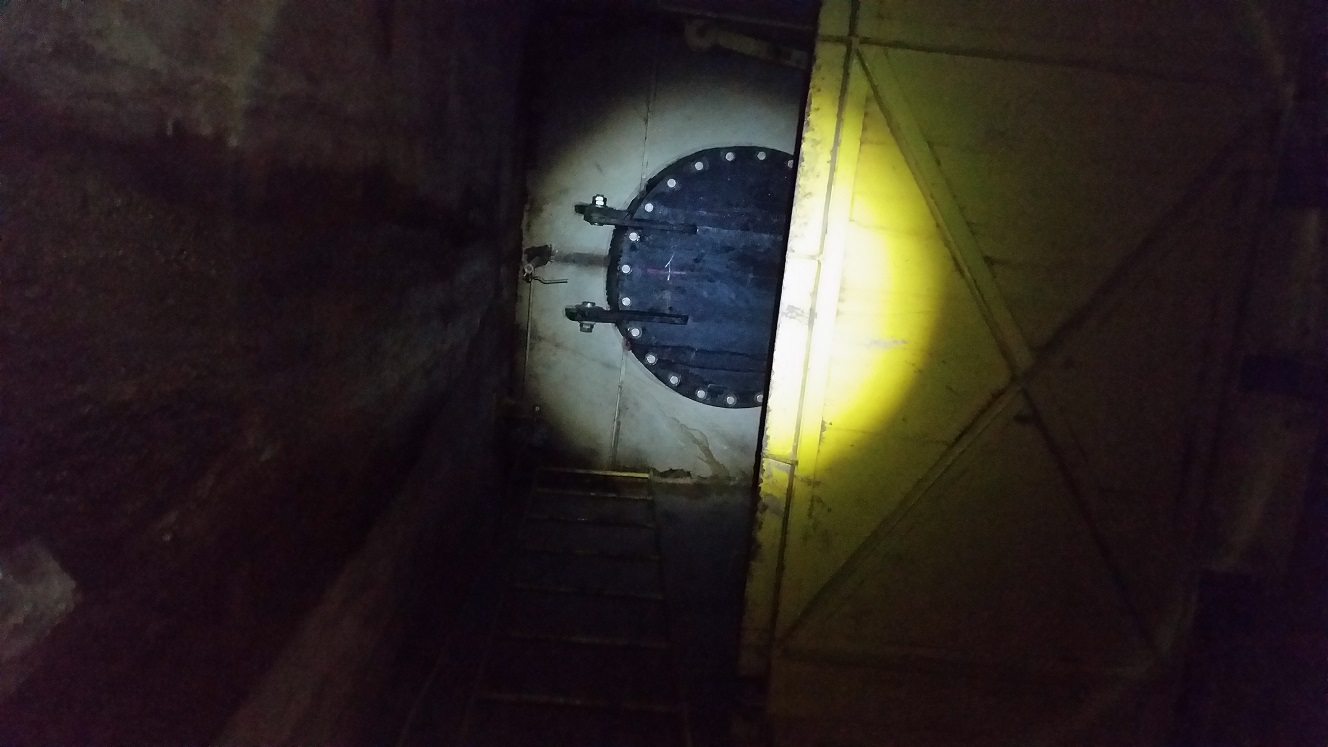
\includegraphics[width=0.8\columnwidth]{figs/bighatch.jpg}
	\caption{The big hatch}
	\label{big_hatch}
\end{figure}
\begin{itemize}
  \item Diameter: $800 mm$ 
\end{itemize}
}

\subsection{Environment constraints}
\frame{
\frametitle{Environment}
\begin{figure}[h!]	
	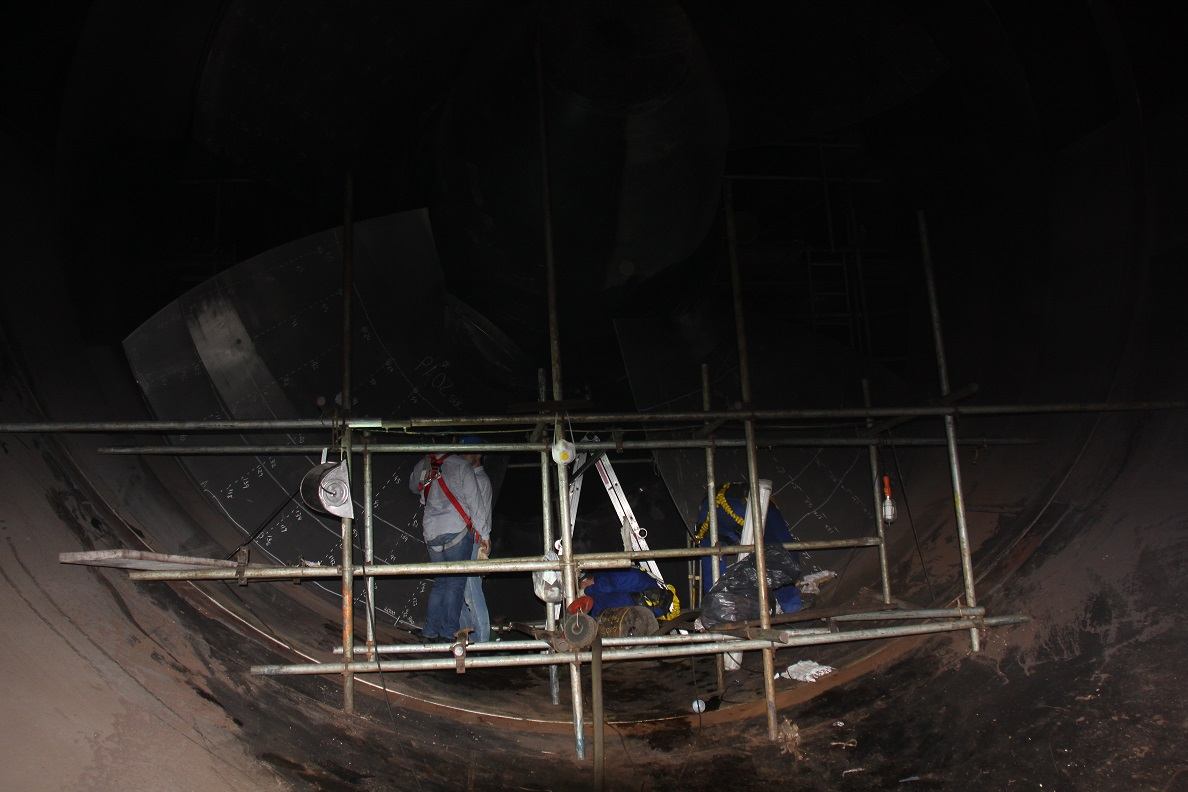
\includegraphics[width=0.6\columnwidth]{figs/environment.jpg}
	\caption{Aro Camara}
	\label{aro_camara}
\end{figure}
\begin{itemize}
  \item Hoist $5 m$;
  \item Slippery and sloping floor;
  \item Dark and damp;
\end{itemize}
}

\section{Pros and cons}

\frame{
\frametitle{Pros and cons} 
\begin{itemize}
  \item Pros
  \item Cons
\end{itemize}
%\begin{block}{Something important}
%Einstein's formula
%$$E=mc^2$$
%\end{block}
}
\subsection{Pros}
\frame{
\frametitle{Pros} 
\begin{itemize}
  \item Mounted small robots or unmounted big robots could pass through hole;
  \item Dry operation;
  \item Free access;
  \item \textbf{Hatch already used for turbine maintenance}.
\end{itemize}
}

\subsection{Cons}
\frame{
\frametitle{Cons} 
\begin{itemize}
  \item Not big enough for mounted big robots;
  \item Complex transportation: scaffolding and hoist;
  \item Difficulties for robot positioning and movement.  
\end{itemize}
}

\section{Logistics solutions}
\frame{
\frametitle{Logistics solutions}
\begin{itemize}
  \item Aro Camara access, robot placement and movement;
\end{itemize}
}

\subsection{Aro Camara access}

\frame{
\frametitle{Aro Camara access}
\begin{figure}[h!]	
	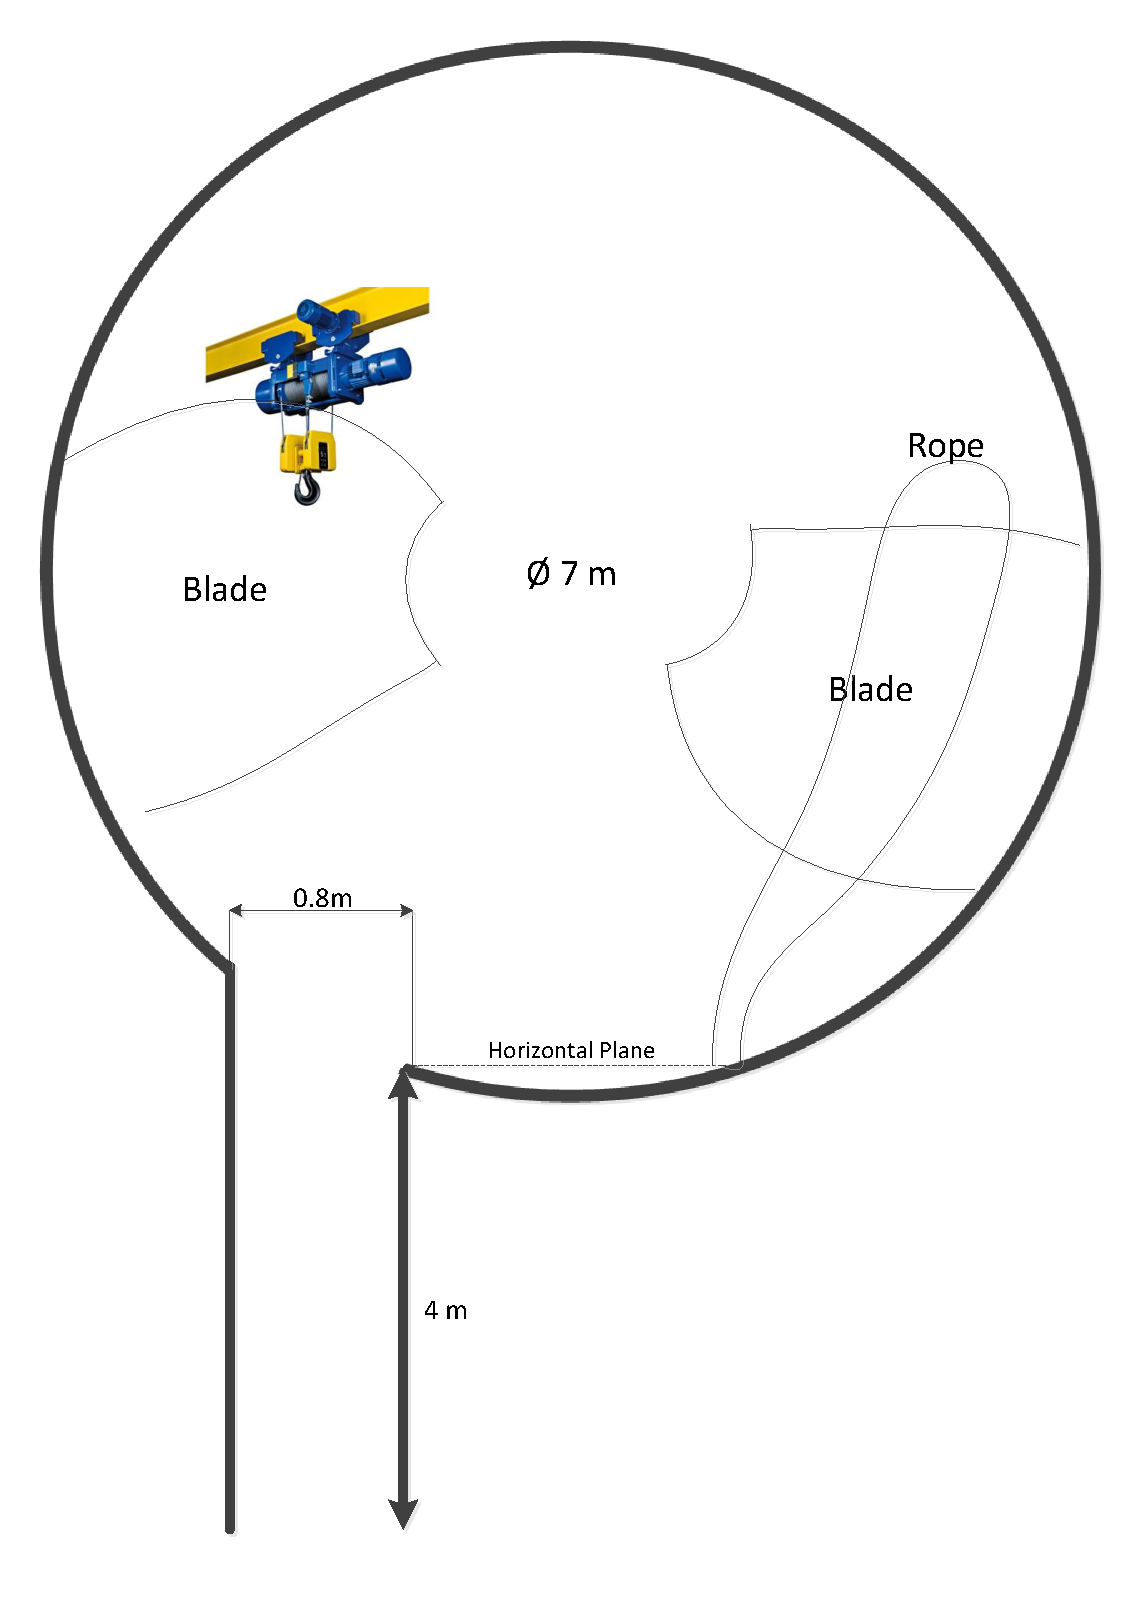
\includegraphics[height=0.45\columnwidth]{figs/Logistics.pdf}
	\caption{Logistics}
	\label{logistics}
\end{figure}
\begin{itemize}
  \item Hoist for robot access;
  \item Scaffolding, wood and ropes;
  \item Robot's base with wheels.
\end{itemize}
}
\frame{
\frametitle{Aro Camara access}
\begin{figure}[h!]	
	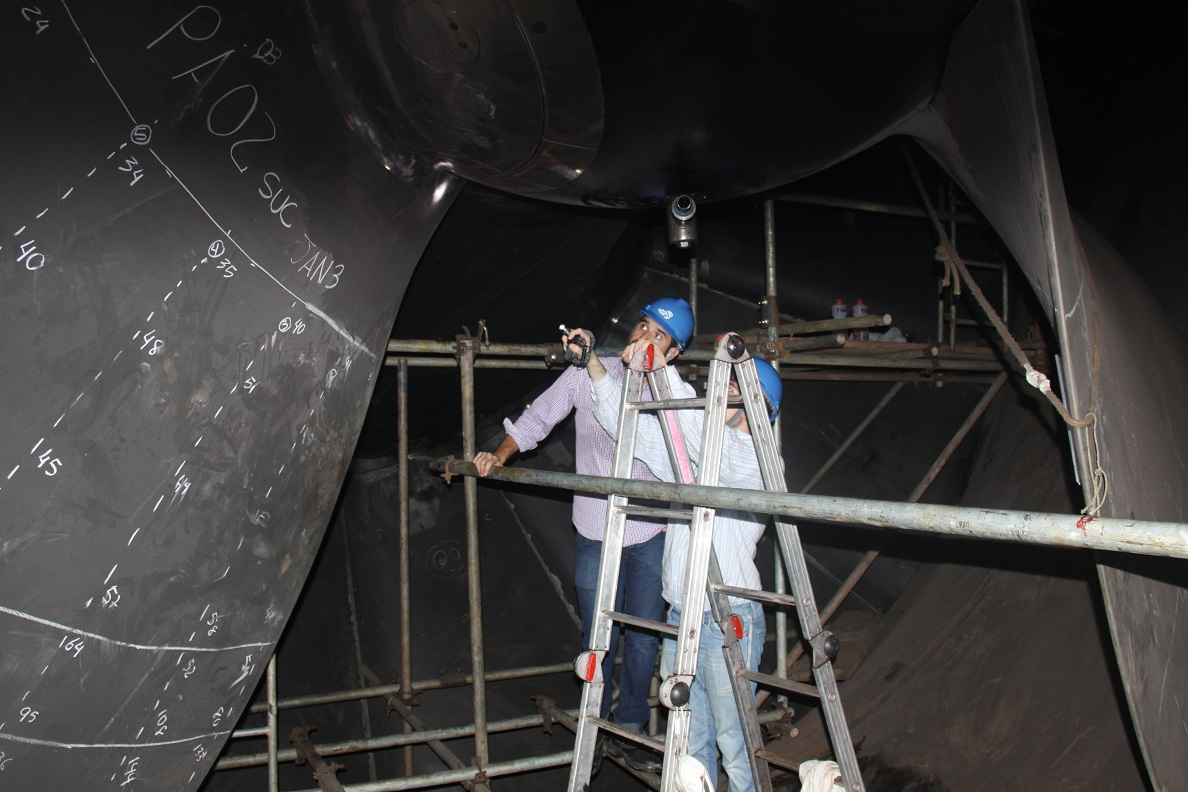
\includegraphics[width=0.9\columnwidth]{figs/ropes.jpg}
	\caption{Scaffolding and ropes}
	\label{ropes}
\end{figure}
}


\subsection{Robot placement and movement}

\frame{
\frametitle{Robot placement and movement}
\begin{itemize}
  \item Pushing and pulling;
  \item Screws on horizontal plane.
\end{itemize}
}

\section{Robotic solutions}
\frame{
\frametitle{Robotic solutions}
\begin{itemize}
  \item Manipulator arm;
  \item Rail robot.
\end{itemize}
}

\subsection{Manipulator arm}
\frame{
\frametitle{Manipulator arm}
\begin{itemize}
  \item Between blades;
  \item In front of the blade.
\end{itemize}
}
\frame{
\frametitle{Between blades}
\begin{figure}[h!]	
	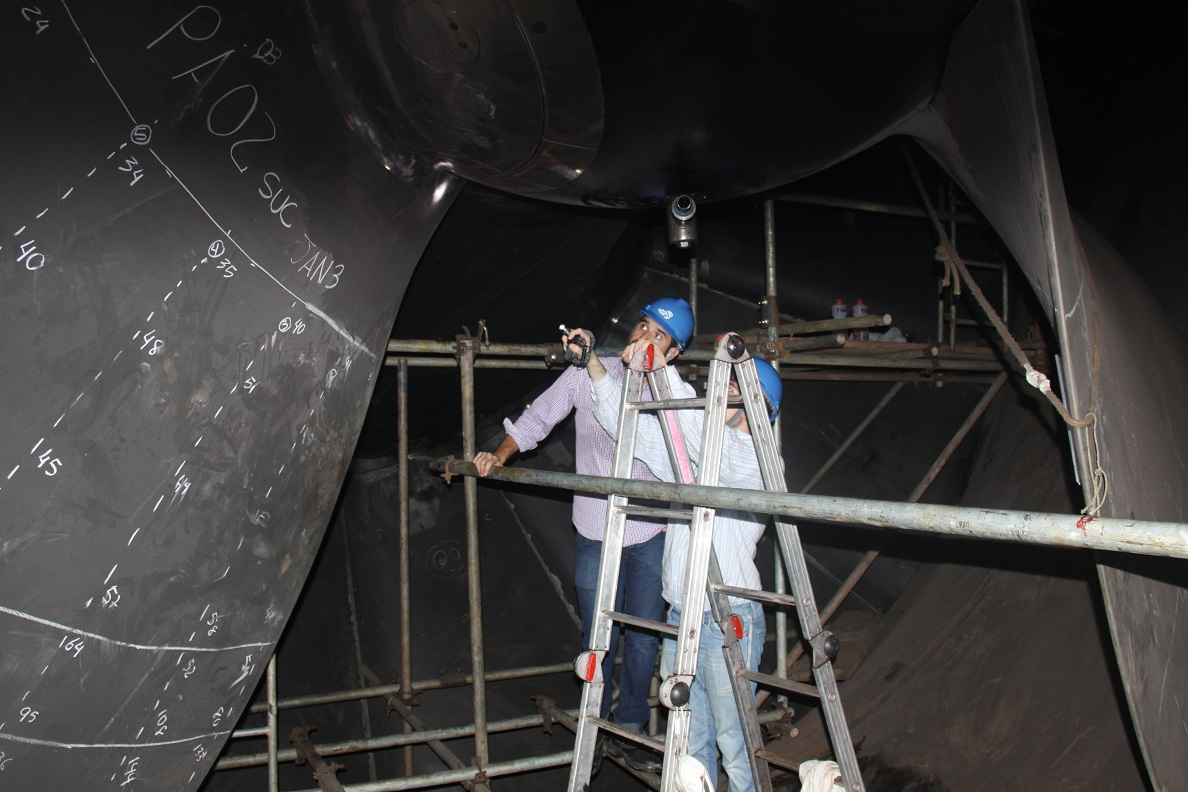
\includegraphics[height=0.6\columnwidth]{figs/between.jpg}
	\caption{Manipulator between blades}
	\label{between}
\end{figure}
}

\frame{
\frametitle{Between blades}
\begin{figure}[h!]	
	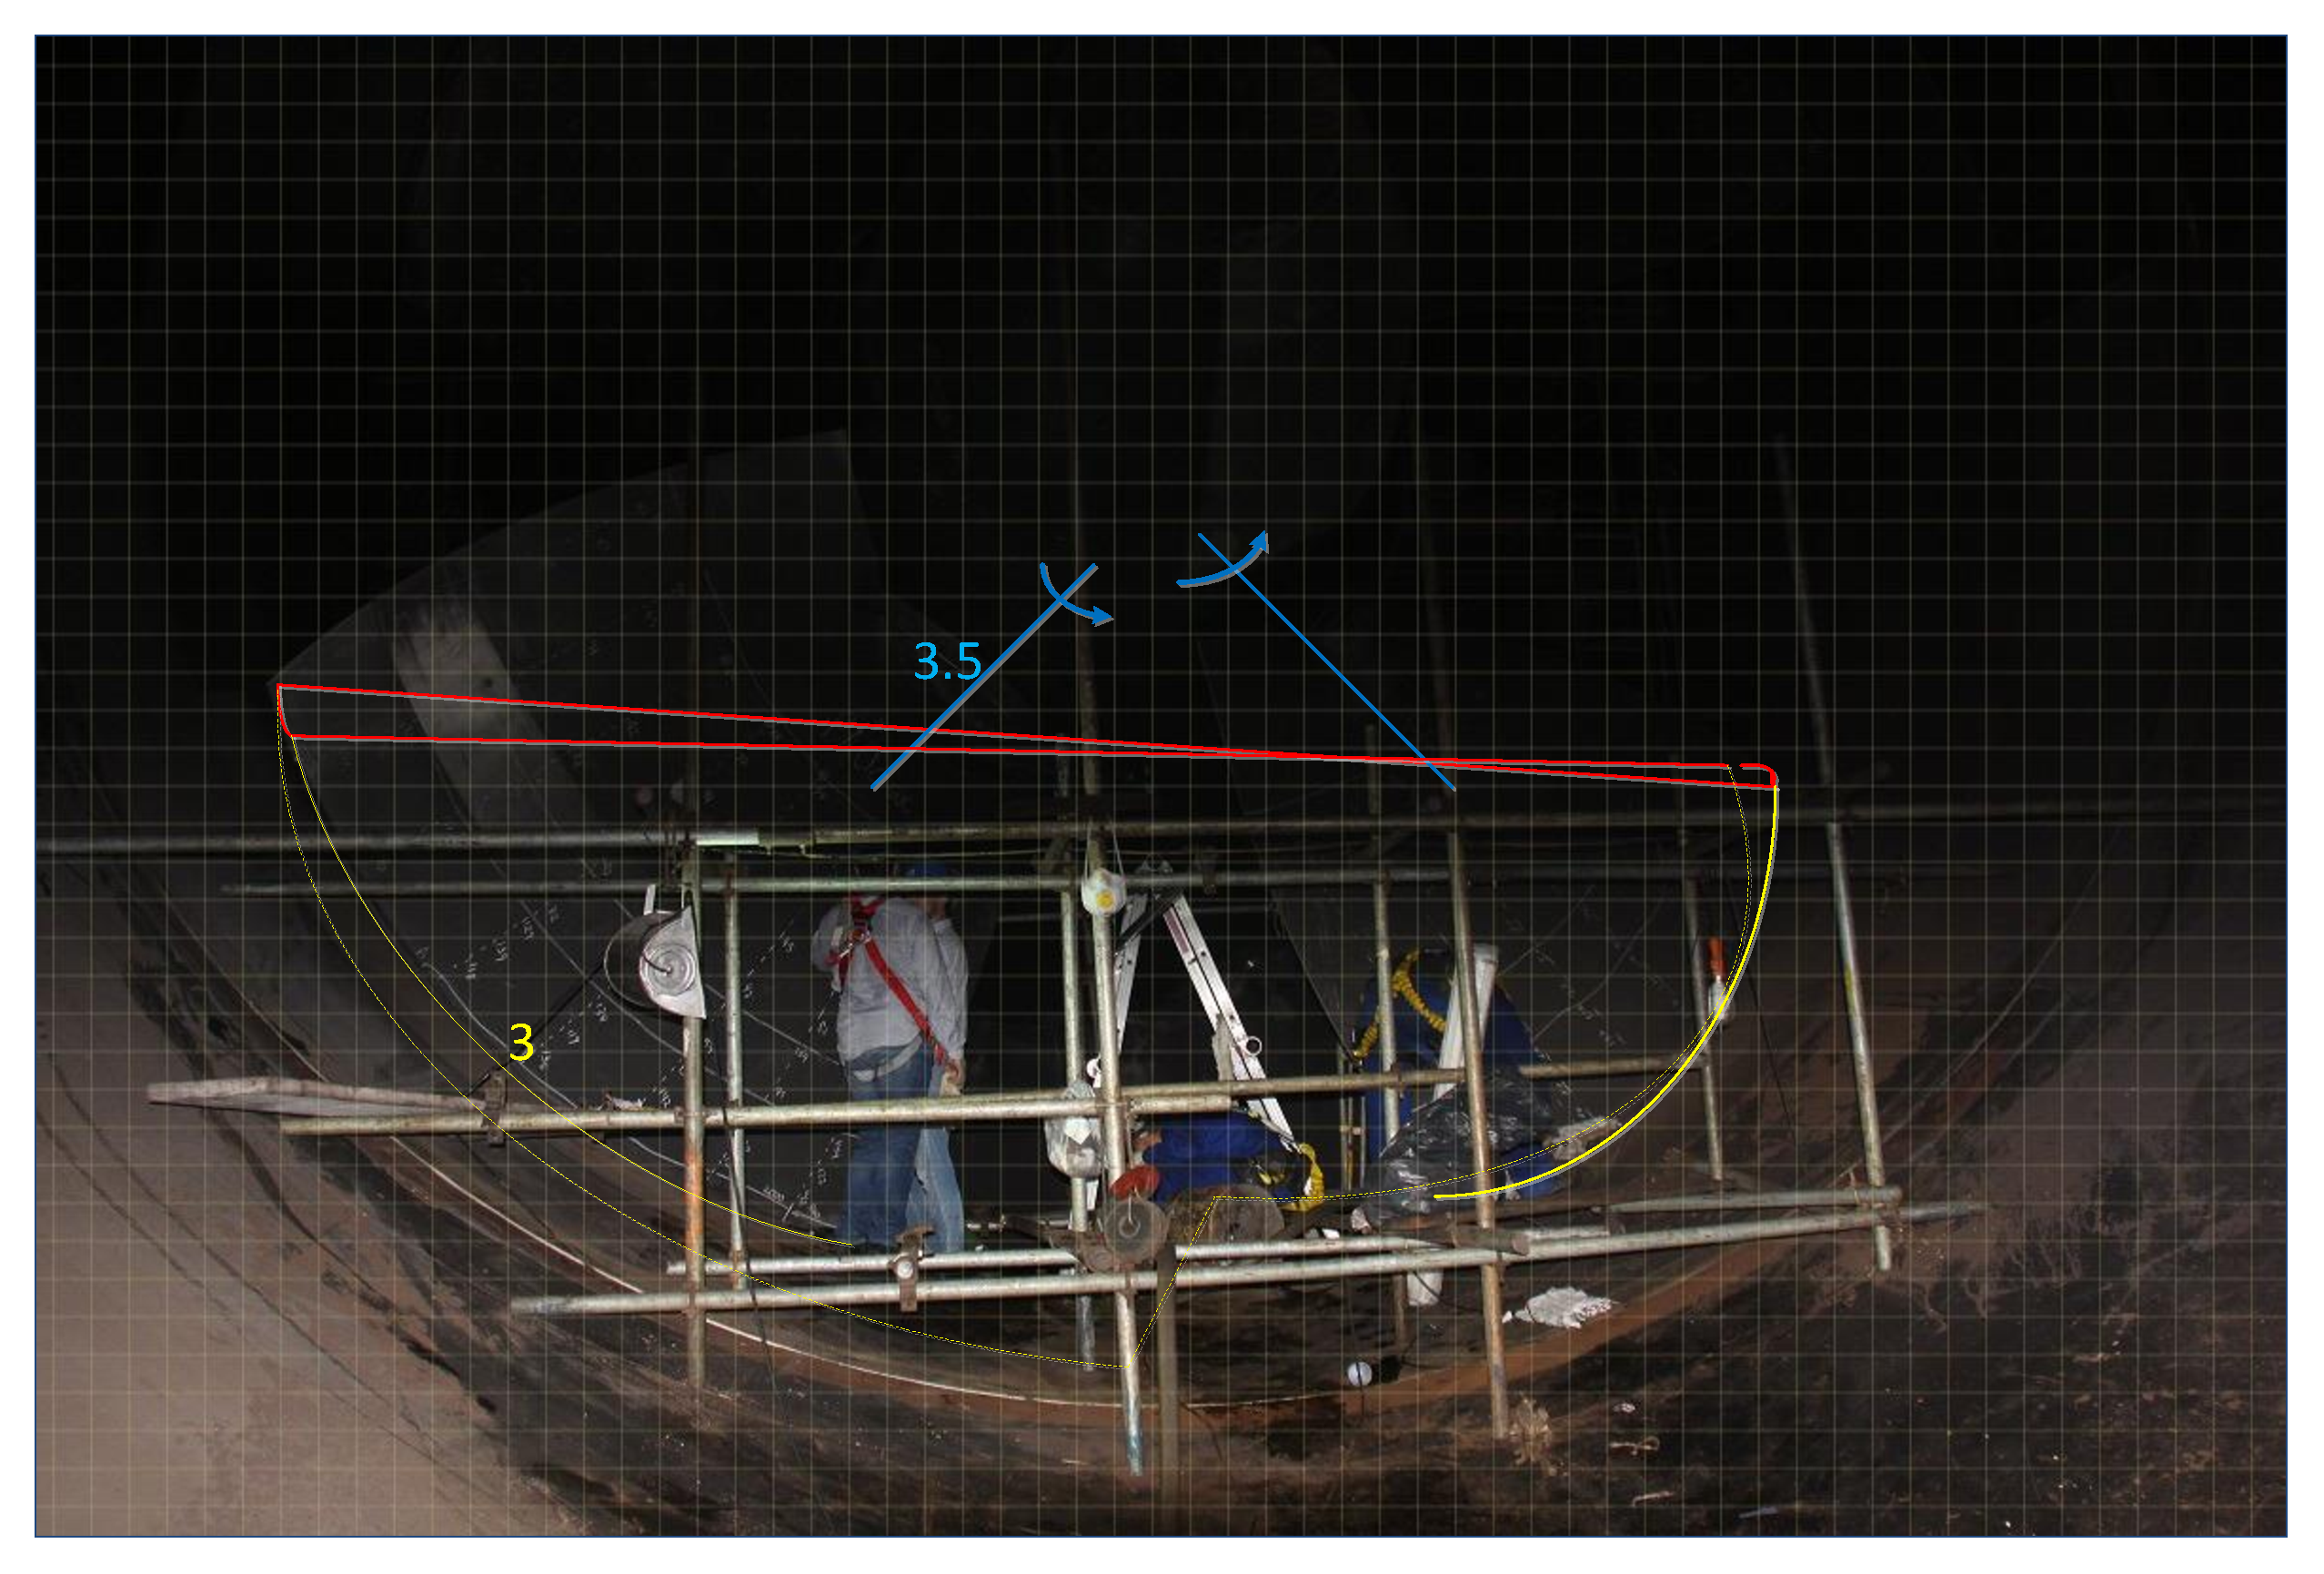
\includegraphics[height=0.4\columnwidth]{figs/envgrid.pdf}
	\caption{Manipulator between blades} 
	\label{between}
\end{figure}
\begin{itemize}
  \item Assuming $3.5 m$ radius;
  \item Base with almost $1 m$ heigth;
  \item Arm must reach $3.5 m$.
\end{itemize}
}

\frame{
\frametitle{Between blades}
\begin{figure}[h!]	
	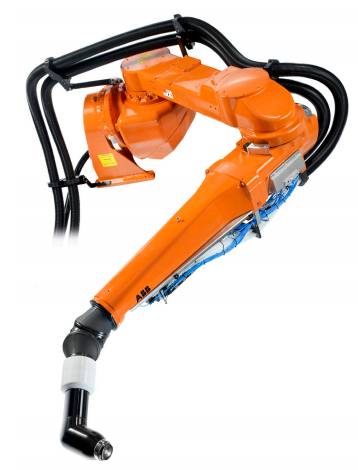
\includegraphics[height=0.38\columnwidth]{figs/irb5500.png}
	\caption{IRB5500} 
	\label{between}
\end{figure}
\begin{itemize}
  \item Everytime you rotate the turbine, you must move the robot; 
  \item No comercial manipulator avaiable. ABB IRB 5500 with $3 m$ reach and
  $700 mm$ base, $540 Kg$.
\end{itemize}
}

\frame{
\frametitle{In front of the blade}
\begin{figure}[h!]	
	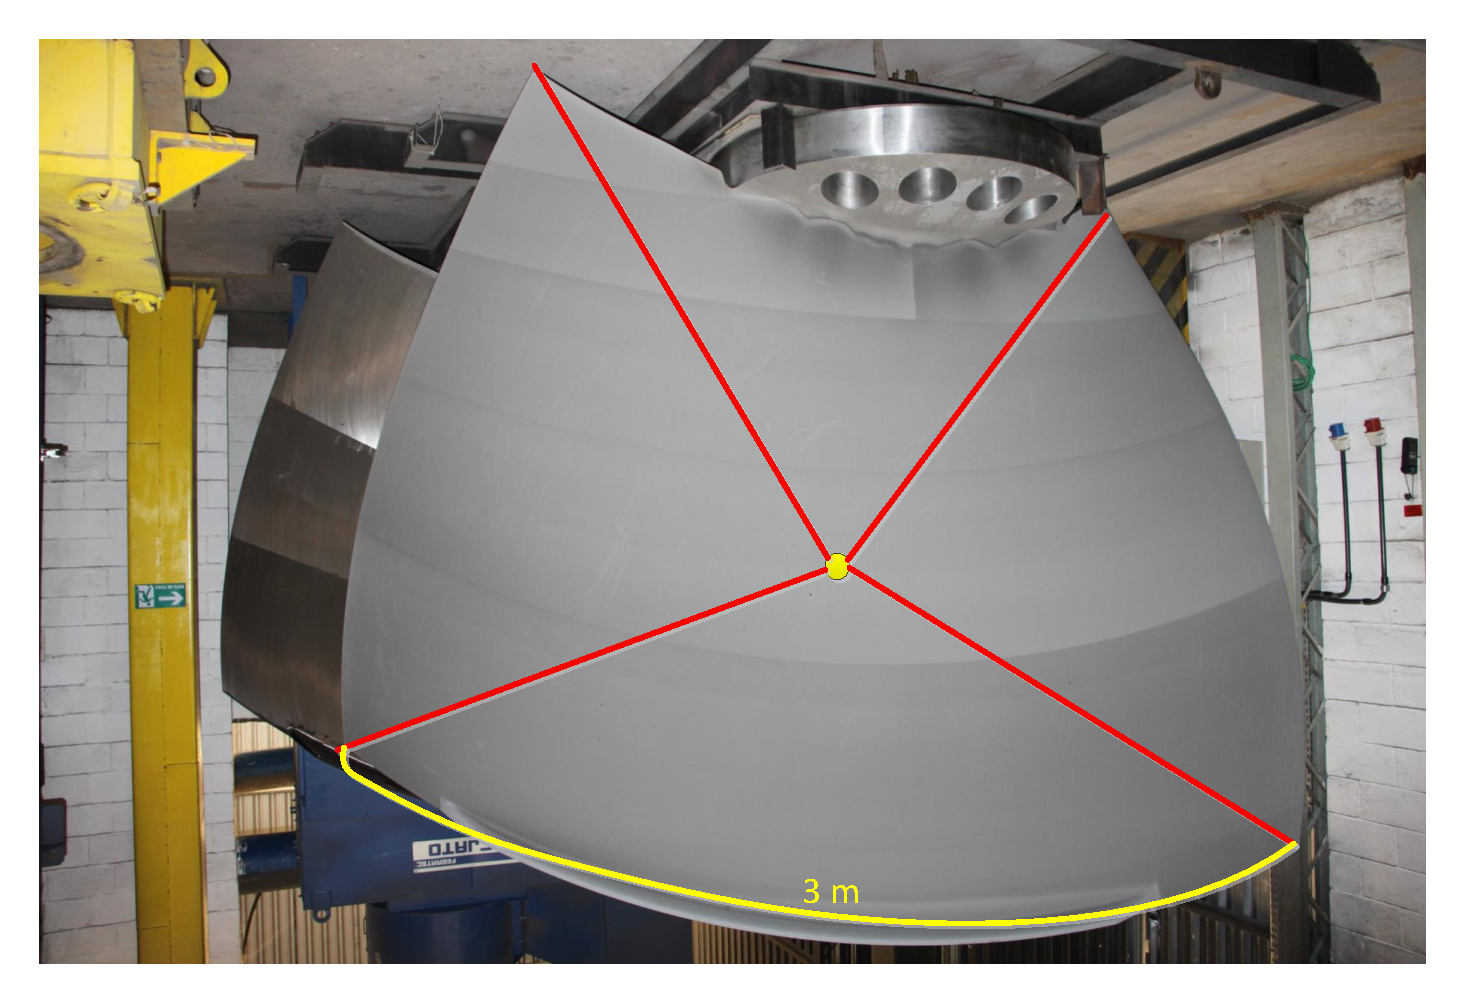
\includegraphics[height=0.4\columnwidth]{figs/bladecalc.pdf}
	\caption{Manipulator in front of the blade}
	\label{infront}
\end{figure}
\begin{itemize}
  \item Assuming $3 m$ arc length;
  \item Base with $1.04 m$ heigth;
  \item Arm must reach $1.67 m$.
\end{itemize}
}

\frame{
\frametitle{In front of the blade}
\begin{figure}[h!]	
	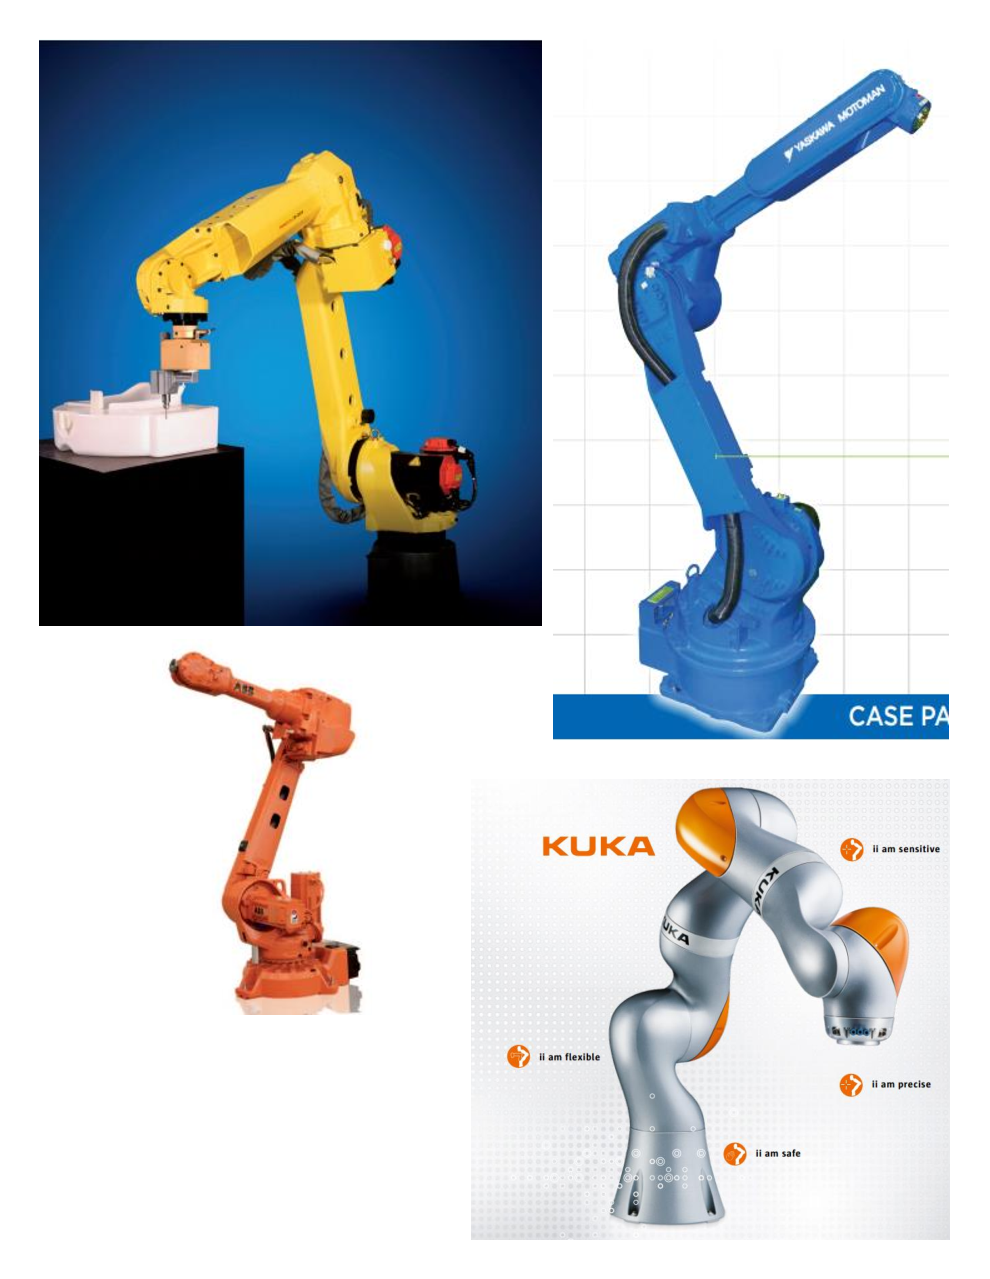
\includegraphics[height=0.4\columnwidth]{figs/arms.pdf}
	\caption{Commercial manipulators}
	\label{commercial}
\end{figure}
\begin{itemize}
  \item Fanuc M-20iA/10L, ABB IRB 2600, Motoman HP20: 250 to 270 Kg robots;
  \item Kuka LBR iiwa 14 R820: 1300 mm reach. Person should not enter the Aro
  Camara after first coating.
\end{itemize}
}

\subsection{Rail Robot}
\frame{
\frametitle{Rail Robot}
\begin{figure}[h!]	
	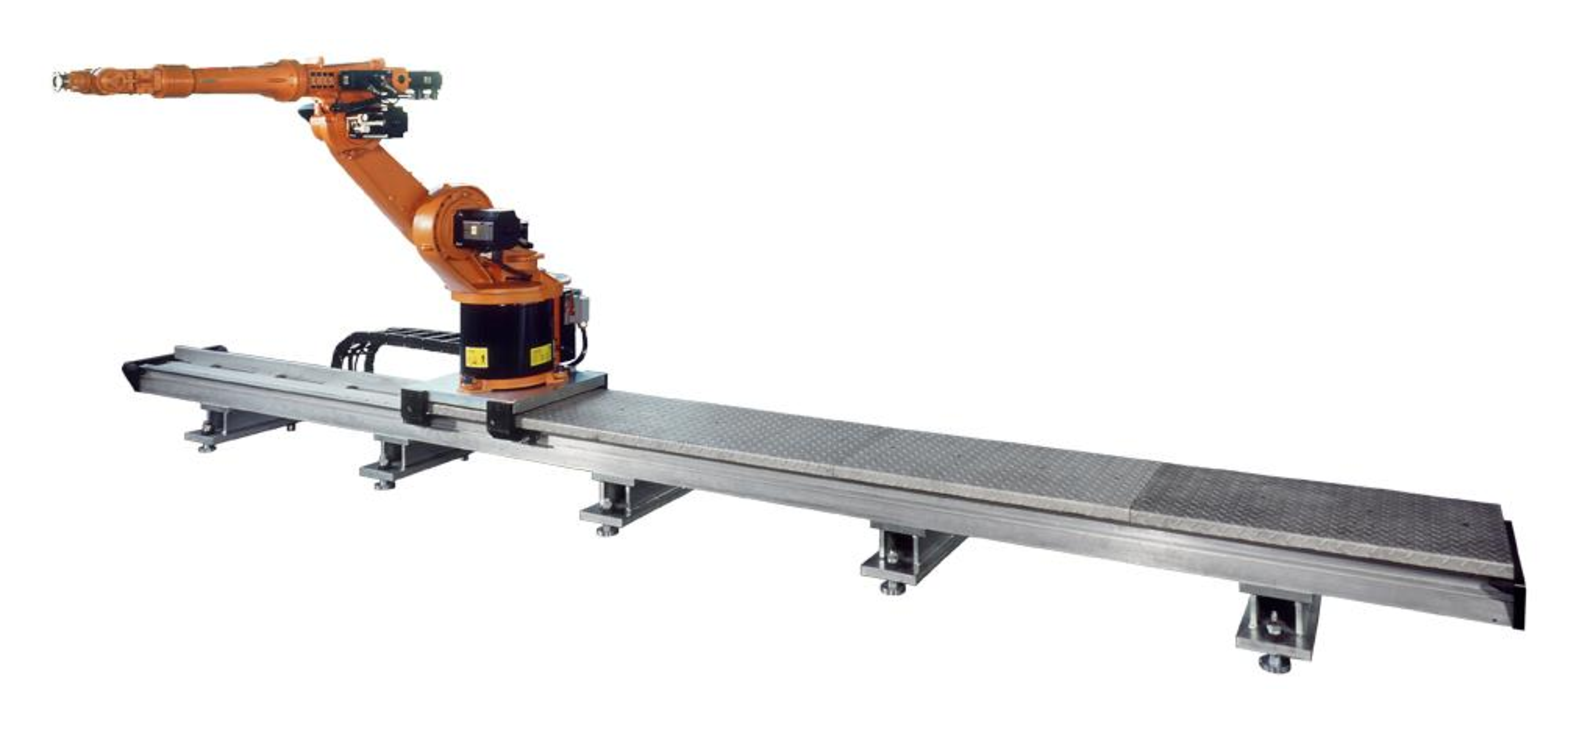
\includegraphics[height=0.5\columnwidth]{figs/rail1.pdf}
	\caption{Manipulator in rail}
	\label{maniprail}
\end{figure}
}
\frame{
\frametitle{Rail Robot}
\begin{figure}[h!]	
	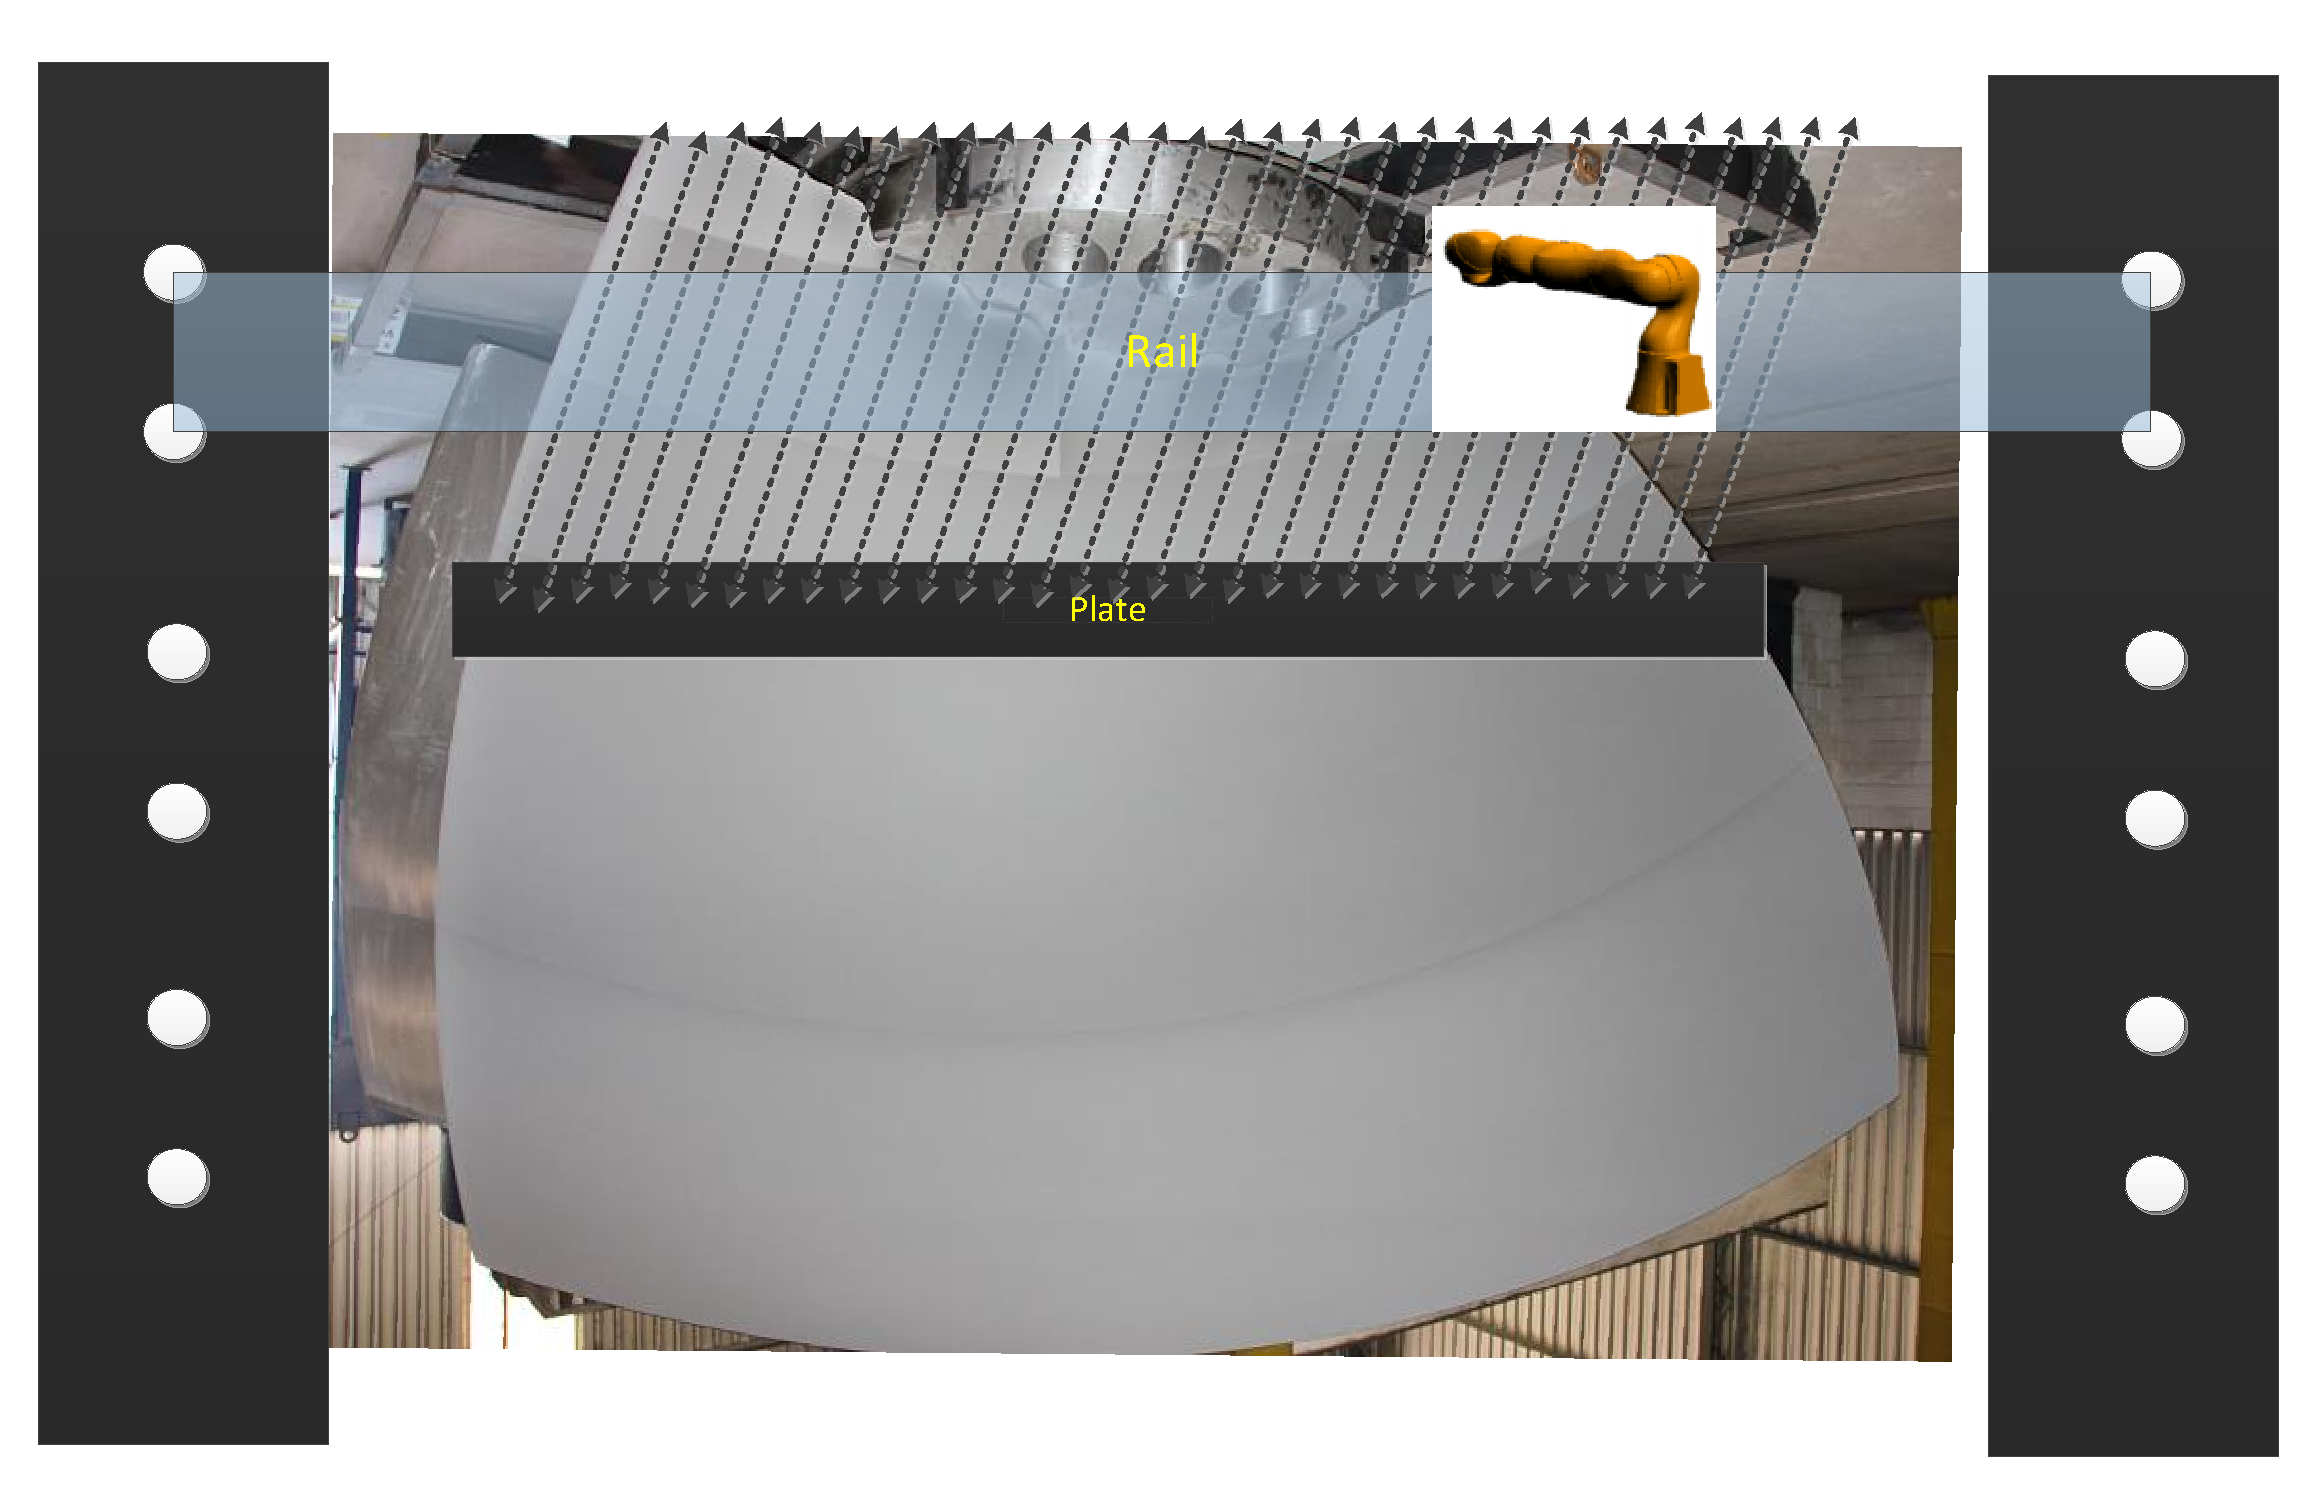
\includegraphics[height=0.6\columnwidth]{figs/rail2.pdf}
	\caption{Rail Concept phase 1}
	\label{bladerail1}
\end{figure}
}
\frame{
\frametitle{Rail Robot}
\begin{figure}[h!]	
	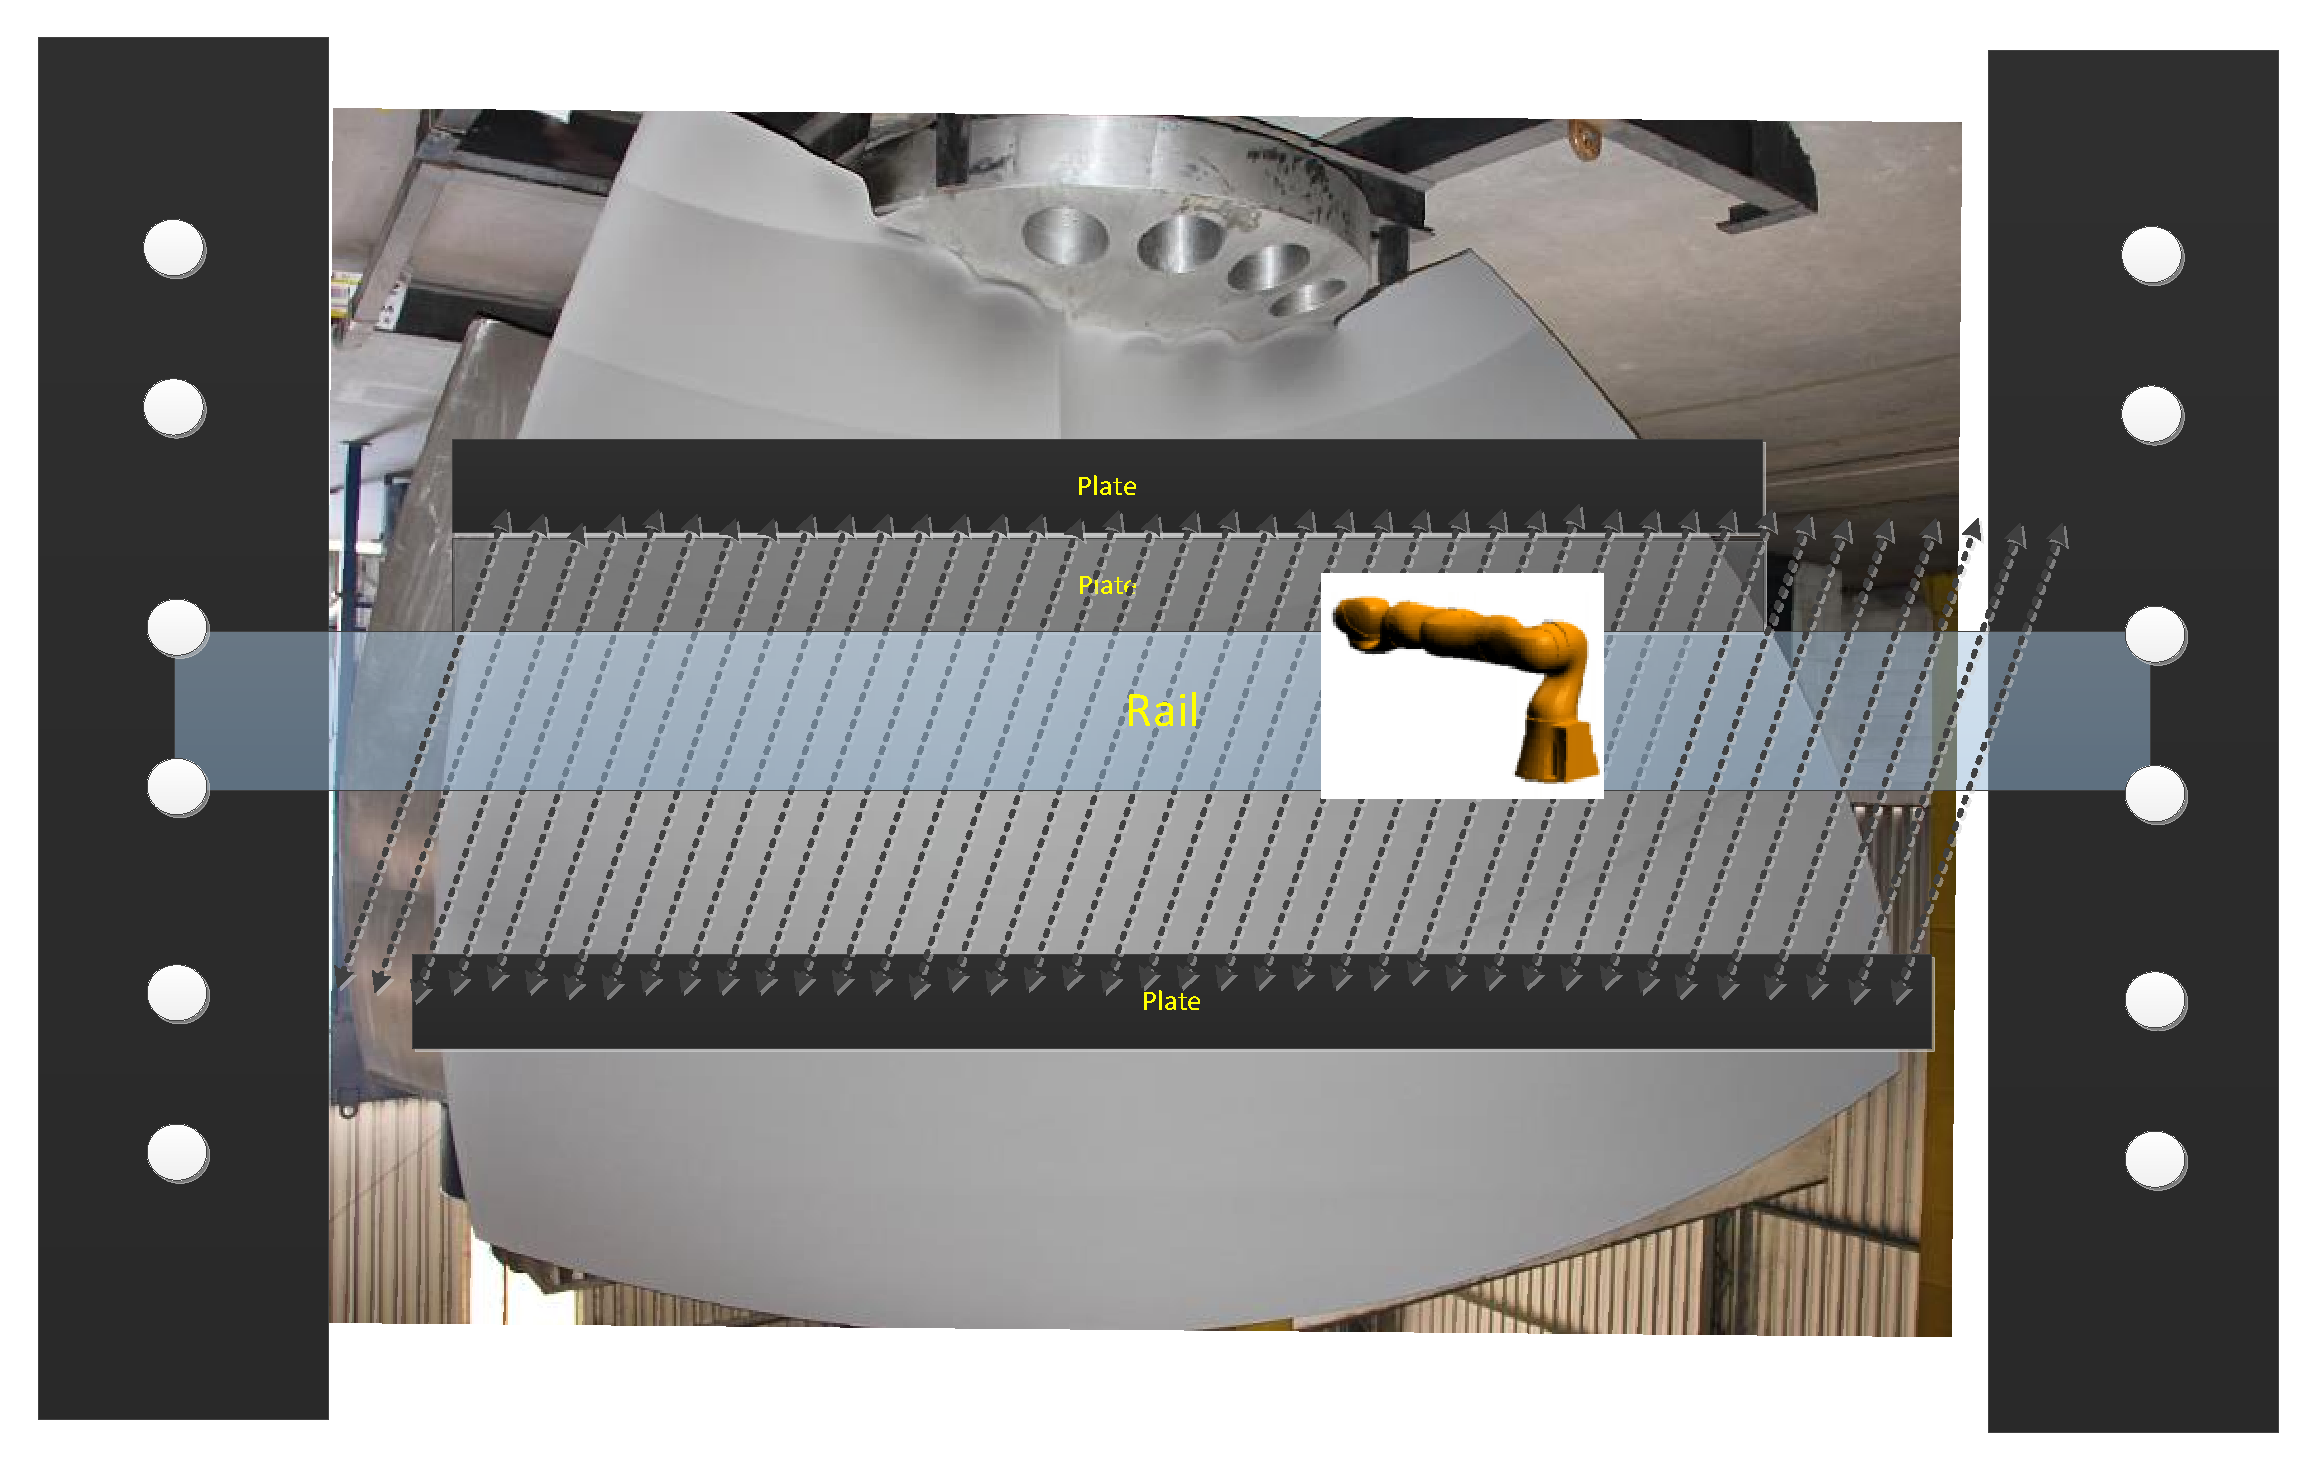
\includegraphics[height=0.6\columnwidth]{figs/rail3.pdf}
	\caption{Rail Concept phase 2}
	\label{bladerail2}
\end{figure}
}
\frame{
\frametitle{Rail Robot}
\begin{figure}[h!]	
	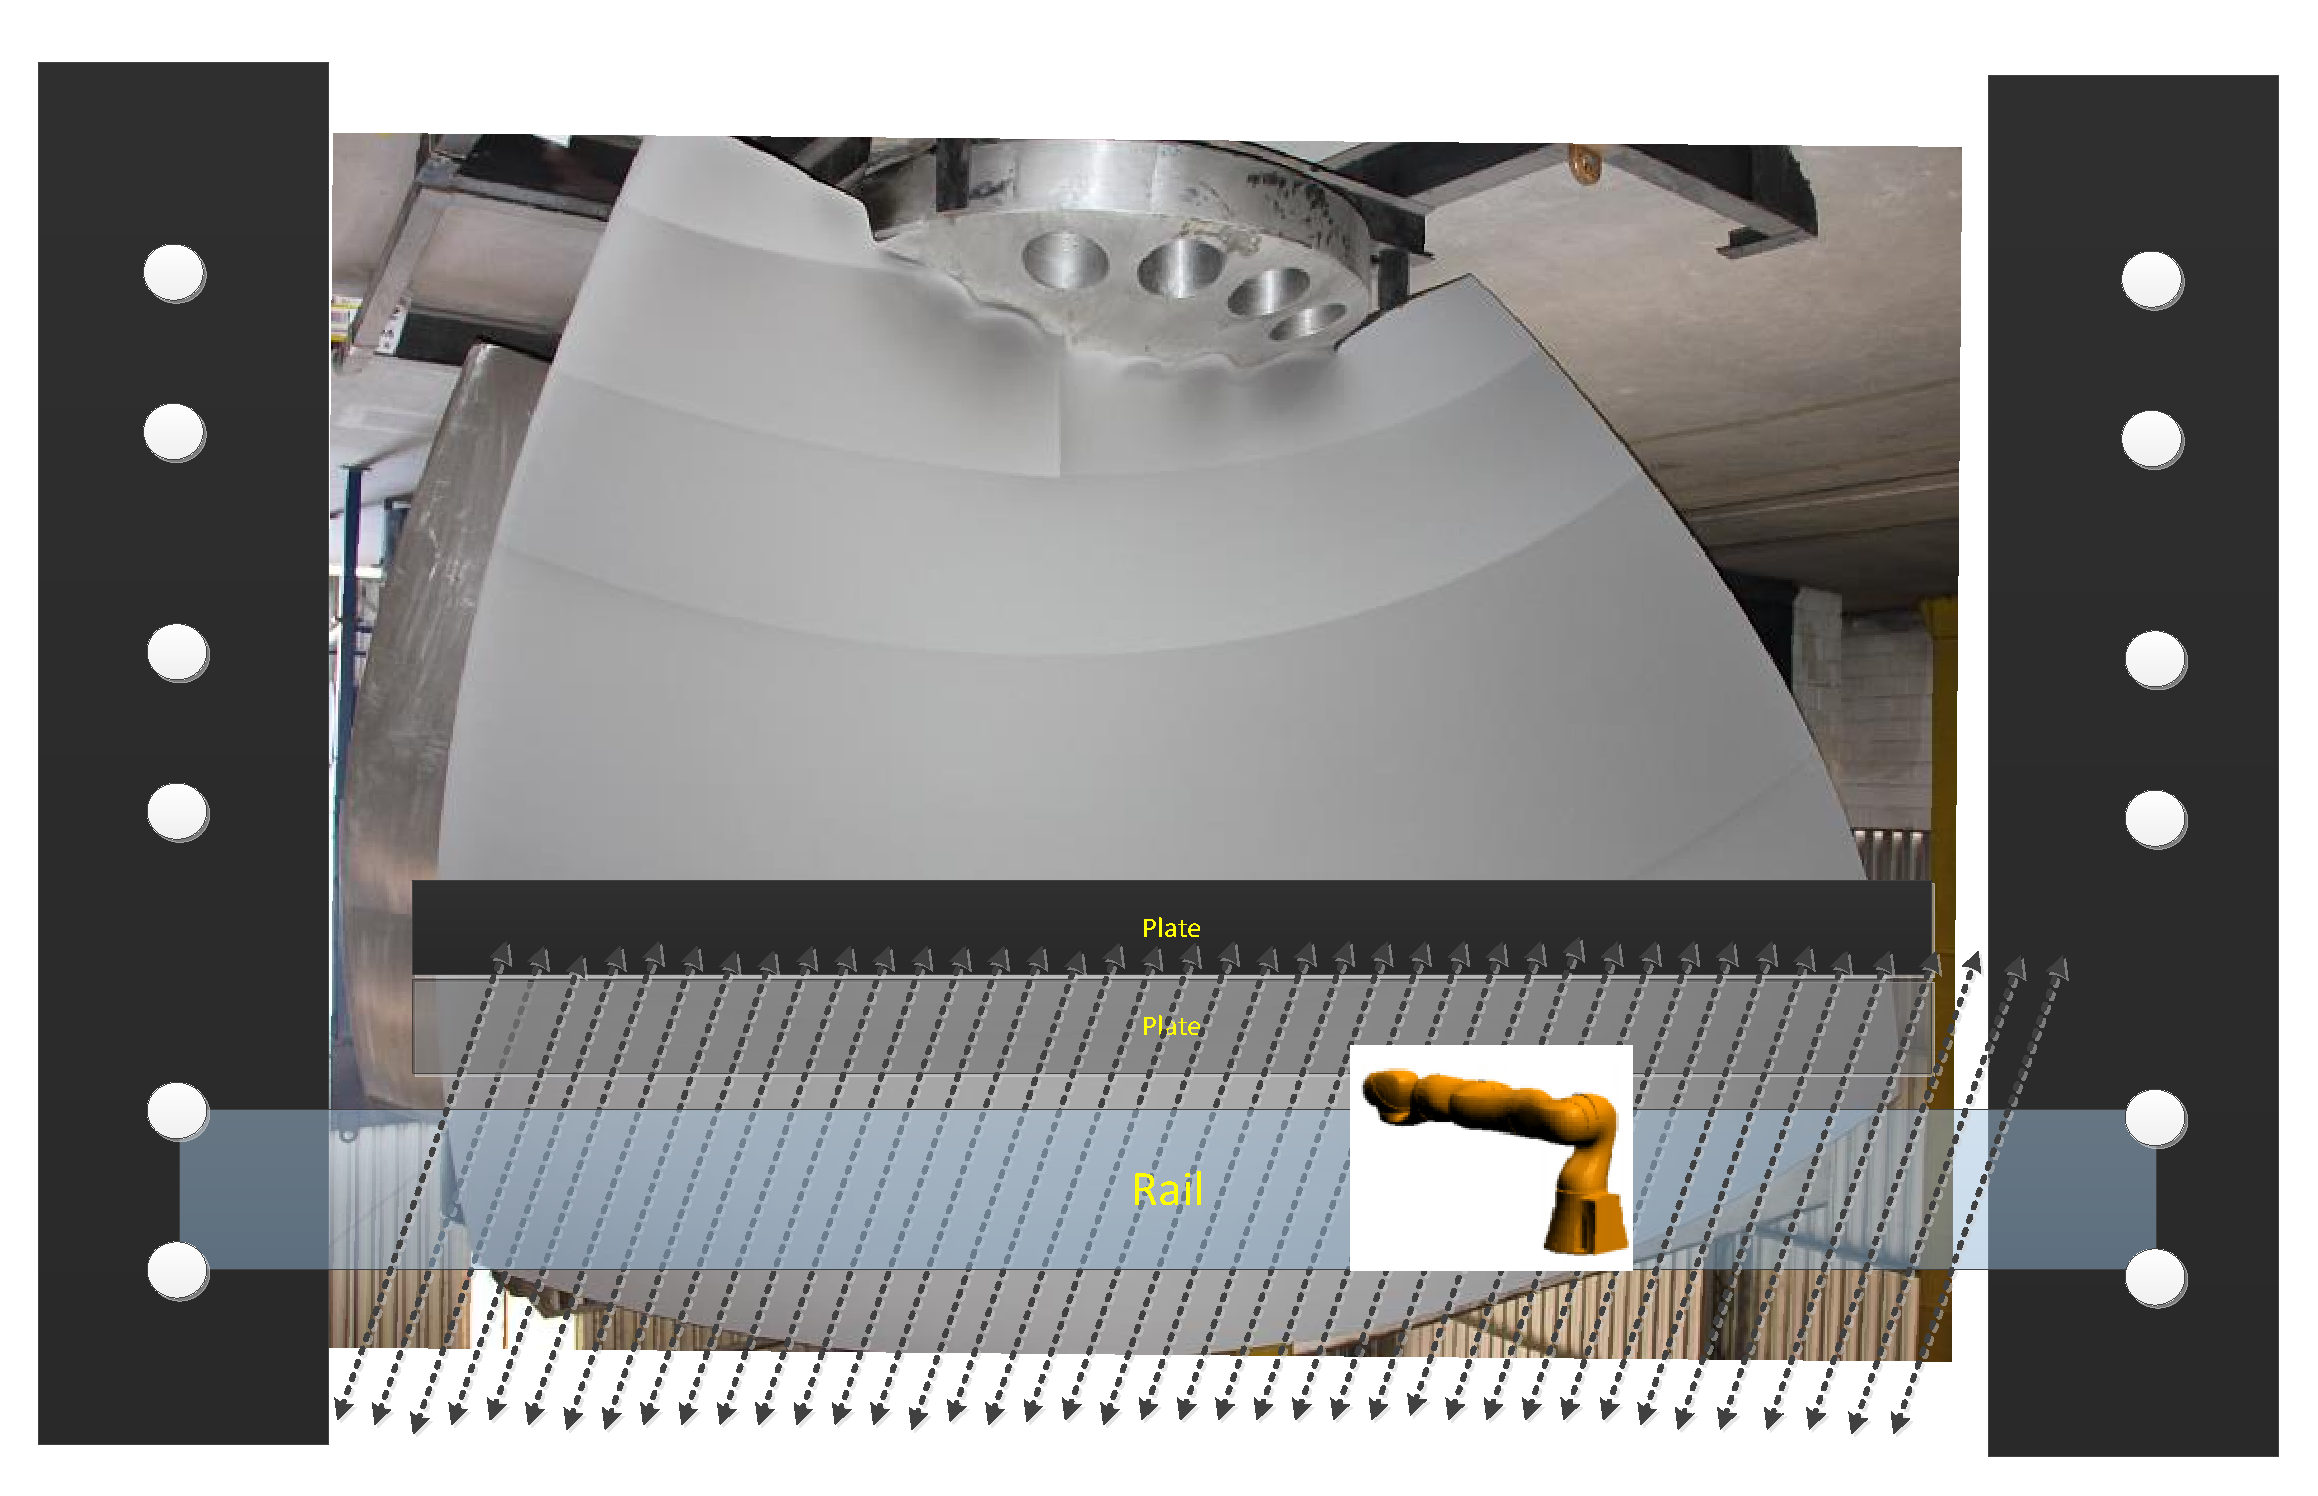
\includegraphics[height=0.6\columnwidth]{figs/rail4.pdf}
	\caption{Rail Concept phase 3}
	\label{bladerail3}
\end{figure}
}
\frame{
\frametitle{Rail Robot}
\begin{figure}[h!]	
	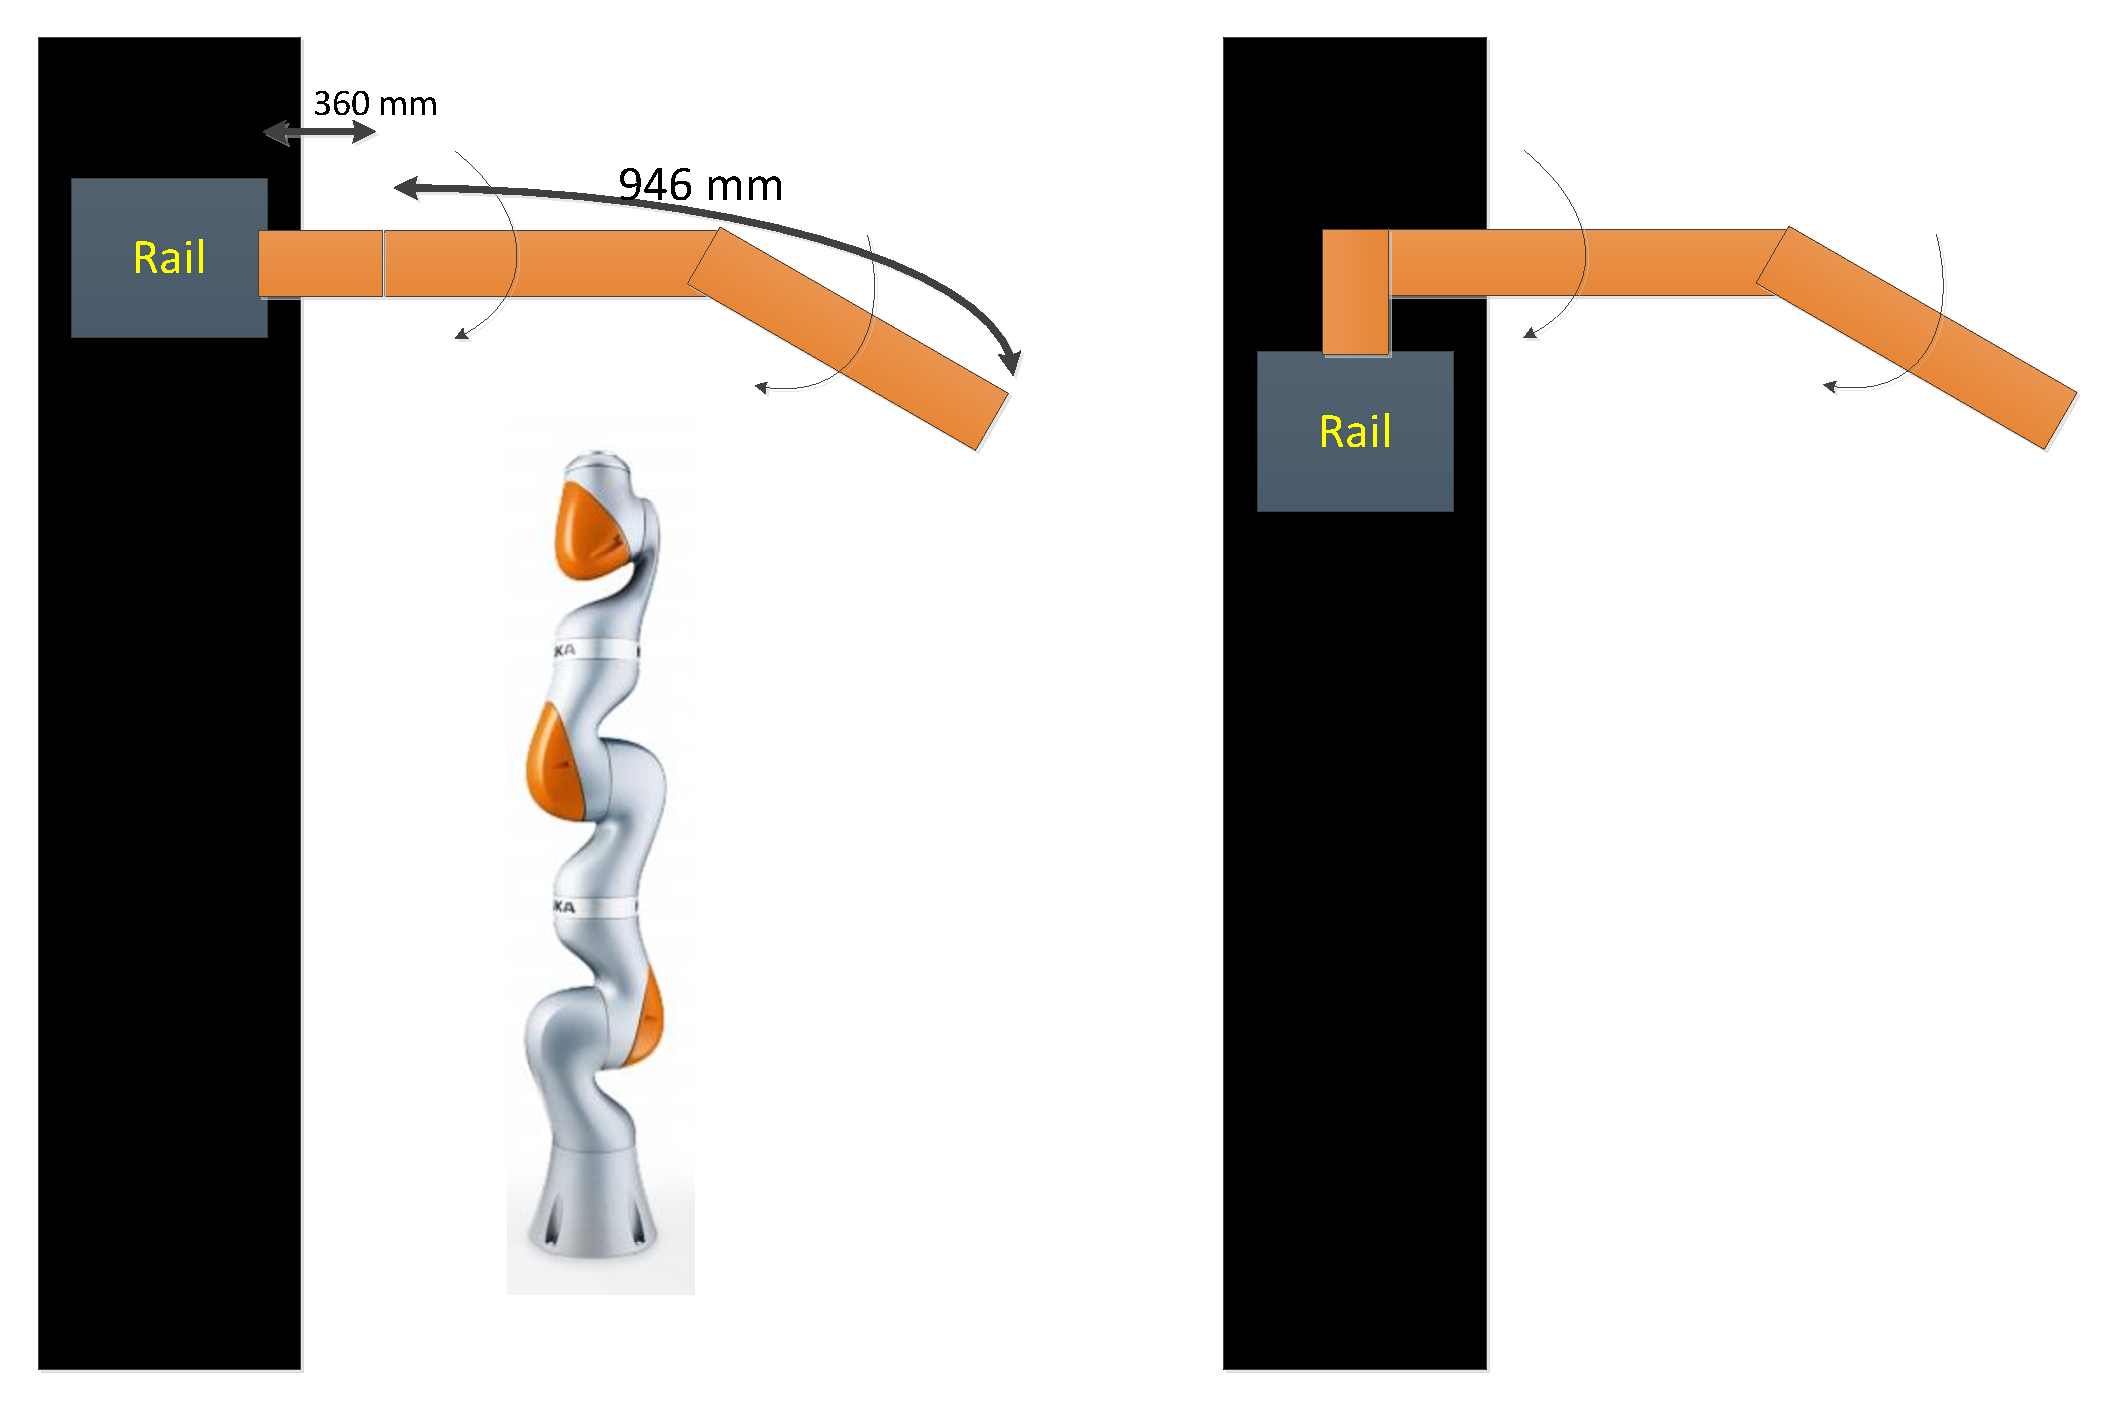
\includegraphics[height=0.6\columnwidth]{figs/rail5.pdf}
	\caption{Rail position}
	\label{railpos}
\end{figure}
\begin{itemize}
  \item Custom rail. Mind torque on rail;
  \item LRB 14 820: $170^o/s$, $940 mm$ end effector, $14 Kg$ payload, $4 Nm$
  end effector torque;
  \item One side of the blade per day. Rail should be mounted and unmounted 4
  times on the other side of the blades.
\end{itemize}
}

\end{document}
